\section{Introduction}

\cut{%%%%%%%%%%%%%%%%%%%%%%
Knowledge empowers the understanding of natural languages.
%The recent emergence of large scale taxonomies and ontologies
%(e.g. WordNet\cite{wordnet}, YAGO\cite{SuchanekKW07},
%TextRunner\cite{BankoCSBE07},
%Google Knowledge Graph\cite{singhal2012:gkg}, Probase\cite{WuLWZ12}, etc.)
%has demonstrated their huge potential in solving natural language
%processing problems.
%It provides a way to extract
%explicit semantics from plain text which is more representative
%than the traditional statistical learning based methods.
%\KZ{Most existing work focuses on extracting noun-concepts in text.
%But verbs play central role in the semantics of sentences.}
Most existing work on text
understanding\cite{GabrilovichM07:ESA,Song11:Conceptualize}
focuses on the semantics of nouns or noun phrases and leverages
popular noun-centric knowledge bases (e.g., YAGO\cite{SuchanekKW07},
TextRunner\cite{BankoCSBE07}, Google Knowledge Graph\cite{singhal2012:gkg},
and Probase\cite{WuLWZ12}), to transform texts into an (often) weighted
list of noun concepts or entities.
%Work in this direction maps the nouns or noun phrases in text to the
%concept space of Wikipedia and Probase respectively. Consequently,
%the representation of the text is converted into a (usually) weighted
%list of concepts.
However, capturing nouns can be insufficient in understanding
a sentence. Consider the following two examples:
%\begin{example}
%\label{eg:acq}
%Company A buys Company B.
%\end{example}
%\begin{example}
%\label{eg:purchase}
%Person C buys a cup of coffee.
%\end{example}
\begin{example}\label{eg:wear1}
mary didn't \underline{wear} {\em the ring} today.
\end{example}
\begin{example}\label{eg:wear2}
mary is \underline{wearing} {\em pink} today.
\end{example}
%\begin{example}
%\label{eg:entertain}
%{\em johnson} is \underline{playing} {\em the lord of the ring}.
%\end{example}
%\begin{example}
%\label{eg:performance}
%{\em mckellen} \underline{played} {\em gandalf}.
%\end{example}
%
Both ``the ring'' and ``pink'' are ambiguous terms.
Without the verb ``wear'', ``the ring'' can refer to either
a decorative accessory, a novel or a horror movie,
while ``pink'' can be anything from
a color, a style, a popular singer, an Aerosmith song,
a Korean movie to a magazine.
%
%Most existing noun-based knowledge bases probably can tell you
%that ``johnson'' and ``mckellen'' are persons.
%Then depending on
%the scale and completeness of the knowledge, they might also know that
%``the lord of the ring'' is a novel or a movie,
%while ``gandalf'' could be anything from
%a mythical dwarf, an airline company, to a music band.
%Without the verb ``play'', it is not easy to determine whether ``the
%lord of the ring'' is a movie or a novel, as ``johnson'' could be reading
%a novel, or watching a movie.
%The situation is worse with the second example as the term ``gandalf''
%is highly ambiguous. This generalized {\em word sense disambiguation} (WSD)
%problem would have been solved, if we knew
%the semantics of the verb ``play.'' For instance, if we knew the verb ``play''
%usually has the following classes of objects: movies, characters, games,
%then we can recognize ``the lord of the ring'' as a movie here and ``gandalf''
%as a character in that movie.
%
%If we only conceptualize the nouns and ignore the verbs in the above examples,
Even if we knew that ``the ring'' is an accessory and
``pink'' is a style, we are still not able to capture the meaning
of the entire sentence, since the noun concepts we obtain from the
two examples are:
\begin{itemize}
\item Example \ref{eg:wear1} $\longrightarrow$ [person] [accessory]
\item Example \ref{eg:wear2} $\longrightarrow$ [person] [style]
\end{itemize}
A person could be {\em buying} an accessory or {\em stealing}
an ornament; and a person could {\em wear}, {\em like} or
even {\em hate} a style. Without specifying the verb
or the predicate, the meaning of the sentence is incomplete.
To fully understand a sentence, one needs to understand the verbs,
in addition to the nouns.
} %%%%%%%%%%% end of cut %%%%%%%%%%%

Verb plays the central role in both syntax and semantics of natural
language sentences. Past research~\cite{mikolov2013efficient,mikolov2013distributed,mikolov2013linguistic} shows that it is
possible to represent the meaning of a word by the distributional
properties of its context, e.g., its surrounding words in a window.
Due to its role in
a sentence, a verb is unique because it maintains dependency relation
with its syntactic arguments such as the subject and the object.
Therefore, it is possible to use the
distribution of immediate arguments of a verb
to represent its meaning~\cite{Levy-acl14}. Such an approach is a form of
``bag-of-words'' (BoW) approach. The common criticisms of the BoW approach
are i) perceived orthorgonality of all words despite some of them share similar
meanings; ii) its high dimensionality and high cost of computation; and
iii) poor readibility to humans.

To ameliorate these limitations, a natural solution is to represent the
arguments by their abstract types, rather than the words themselves.
It is reasonable to assume that a verb represents different meanings,
or different senses, if it's used with different types of arguments.
To that end, FrameNet\cite{baker1998berkeley} and VerbNet\cite{KipperDP00}
are all examples of human-annotated lexicons that include verbs and their
meanings (called {\em frames}) and the different types of
their arguments (called {\em thematic roles} or {\em semantic roles}).
Due to the excessive cost of constructing such
lexicons, as well as their intentional shallow semantic nature,
the abstraction of verb arguments is very coarse-grained. For example,
in FrameNet, the verb ``eat'' has just one frame, namely ``Ingestion'',
and its direct object has just one role, ``Ingestibles.''
%Such abstraction,
%though human readable, is not very helpful in capturing the full semantics
%of the verb in computation.
Furthermore, the lexical coverage of these
resources are very limited. FrameNet, which is the most popular and best
maintained among the three, consists of just 3000 verbs and 1200
frames.


%
%
%One way to understand the semantics of a verb is to analyze
%the semantic classes or types of its main arguments
%such as the subject or the direct object. A verb represents different meanings,
%or different senses, if it's used with different types of arguments.
%For example, a person playing a movie
%means {\em entertainment} while a person playing a character means
%{\em acting}.
%In the first sentence, conceptualizing on nouns results in a concept
%``company'' with strong confidence, because there are only
%two nouns in the sentence: Company A and Company B.
%But ``company'' is not a proper concept to summarize the semantic
%of the sentence in this scenario.
%In the second sentence, conceptualizing on nouns is not able to tell
%whether this sentence is about ``person'' or ``drink''.
%The verb ``buy'' in both of the sentences acts an
%important role of modifying the semantics. According to different
%subjects and objects, the verb makes the sentences different in
%semantics. The first ``buy'' is company acquisition while the
%second one is purchase. This phenomenon shows the importance of
%verb lexicons in semantic analysis.
%
%\KZ{SRL requires manually curated lexicons and is
%too coarse-grained.}
%Semantic Role Labeling (SRL) is one important technique toward that goal.
%It captures the semantics of verbs/predicates by automatically identifying
%the sense of a verb (known as a {\em frame}) and
%annotating the {\em roles} of the arguments of that verb.
%%In Example \ref{eg:performance},
%%``play'' is used as the ``Performers\_and\_roles'' frame, while the
%%role of {\em gandalf} is ``Role''.
%In SRL, the definitions of the frames
%and roles are specified, usually manually, in a lexicon (e.g.,
%FrameNet\cite{baker1998berkeley}, PropBank\cite{kingsbury2002treebank},
%and VerbNet\cite{KipperDP00}), which comes with
%a number of example sentences annotated with the frames and roles.
%%the semantic role for each verb argument. For example, ``coffee''
%% in \exref{eg:purchase} acts the roles of ``Goods'' in FrameNet.
%However, SRL algorithms are limited to the
%human annotated lexcons, which contains only moderate numbers
%of verbs and frames (3000 verbs and 1200 frames in FrameNet)
%, coarse-grained senses and non-human readable semantic roles (e.g., ``Ingestibles'' for
%the verb ``eat'').

%There are three main limitations of such lexicons.
%First, human annotation is required to produce such lexicons,
%which limits their {\em scales}.
%FrameNet, which is by far the most popular SRL lexicon,
%contains just over 3000 verbs and 1200 frames. % and 13,000 word lexical units.
%Many frequently used verbs/verb phrases,
%such as ``accept'', ``promote'', ``carry out'', are
%not covered by FrameNet, and many verbs have only
%one frame/meaning. Second, the frames are
%{\em coarse-grained} and close senses such
%as ``clothing'' and ``accessory'' for the object of ``wear'' are not
%distinguished by FrameNet. Third, semantic roles
%such as ``Ingestibles'' (object of the verb ``eat'') are
%not popular uttered by ordinary people.

%Many verbs has just one frame or one meaning.
%For example, there is only one frame associated with ``wear'',
%which is ``Wearing'', and its object takes just one role,
%``Clothing''.

%Clearly this frame doesn't apply to Example \ref{eg:wear1},
%since the ring is not clothing by any means.
%It is not suitable to be
%applied to big data that contains verbs or verb senses
%not presented before.

%Second, the frames are {\em coarse-grained}
%in these lexicons, making them unable to tell the
%difference between two close senses.
%For example, the role ``Clothing'' for ``wear'' is
%too coarse-grained to cover the delicate meaning of ``wear''
%in the two examples above.
%A better, and more refined way
%to classify the types of the object of ``wear'' might be
%``clothing'', ``accessory'', ``style'', among others.
%and ``food'', where the last one represents the common ``ingestibles.''
%E.g. ``buy'' has only a role ``Goods'' for its object
%in FrameNet while ``Company B'' is not precisely a ``Goods''.

%Third, semantic roles in SRL are used as {\em labels} only.
%While readable by human, labels like ``Ingestibles''
%(for the verb ``eat'') or
%``Sound\_makers'' (for the verb ``play'')
%are not popular terms uttered by ordinary people.
%so the audience of SRL lexicons is restricted to language researchers.
%Moreover, because such terms don't usually appear in text itself,
%the role names and frame names are not computationally related to each other.
%Therefore, it is not easy to apply such lexicons in automatic computation of
%similarity or summarization.

%\KZ{Our purpose is to provide a generalized concept lexicon for verb
%arguments. This lexicon can help us understand text, detect logical
%errors and make predictions while parsing text. This is more general
%than the data produced by the ReVerb project because we provide abstraction
%of argument types. By conceptualizing the arguments of verbs, we can
%better understand the different semantics of verbs and possible group verbs
%of similar uses together.}
%
%\KZ{In my opinion, our work sits in between SRL and SP. Both of these
%work relate verb/predicate to its argument types. But their focuses
%are a little different. SRL focuses on coarse-grained, shallow semantics
%of verb predicates. The argument types exemplify very coarse grained usage
%(roles) of different verbs (senses). These types are often mutually exclusive
%and human readable but often not machine processible,
%and the scales are limited due to heavy dependence on human labeling.
%SP (or selectional association to be specific) gives the
%likelihood of a semantic class acting as an argument of a verb predicate.
%It's main purpose is to empower WSD with additional semantic information
%from verbs. It can give a ranked list of concepts which are most associated
%with a predicate but it makes no assumption about the mutual exclusion among
%these concepts, (concepts in WordNet do overlap). What we want to achieve
%in this work is to automatically infer the usages of each verb and make them
%human readable as well as machine readable. That's why the definition of
%our problem is to minimize the number of types, while ensuring that the
%overlapping between the types are bounded.}

%There are three kinds of works centered on verb analysis:
%semantic role labeling, ReVerb and selectional preference.
%In semantic role labeling(SRL), nouns or clauses are labeled as
%a functional role to the verb. e.g. Company B is marked as
%the patient of the verb ``buy'' in the previous example.
%However, a semantic role labeler is learnt from a limit set
%of annotated training examples, which makes it impossible to
%handle verbs that are not in the training set. In addition,
%the predefined semantics(e.g. semantic frames in FrameNet)
%of each verb is coarse grained, making it unable to tell the
%difference between two close senses.

%\KZ{ReVerb is too specific and doesn't generalize.}
%If SRL algorithms provide only coarse-grained semantics, then
%ReVerb \cite{FaderSE11} lies on the other end of the spectrum.
%ReVerb is an open information extraction system that discovers
%binary relations\footnote{ReVerb extracts general relations
%instead of verb predicates,
%e.g., XXX {\em heavily depends on} YYY.}
%and the class of the arguments are coarse-grained.
%%their arguments from the web without using any predefined
%%lexicon
%Moreover, although ReVerb contains 15 million subject-predicate-object triple
%instances, but the predicates are often too specific, and thus
%the number of triples for each predicate is limited. For example, the instances
%for verb ``wear'' only contains 324 instances.
%

%Instead, it extracts the relations by a rule-based algorithm.
%ReVerb data contains 15 million subject-predicate-object triple
%instances without any abstraction or generalization.\footnote{ReVerb
%does include ad hoc Freebase \cite{freebase}
%types to categorize the triples on its website, but these
%cannot be used in computation directly.}
%%These types, such as ``art subject'', ``organization classification'',
%%and ``invention'' are not created for any particular argument of
%%the relation and cannot be used in computation directly.
%The lack of abstraction in ReVerb has
%an obvious drawback: a system powered by ReVerb will not recognize a
%verb and its arguments unless it has this triple explicitly stored
%in the knowledge. But to date, the scale of ReVerb is far from sufficient
%to cover all triples that ever appear in text.
%\textcolor{red}{
%The available ReVerb data contains 15 million triples extracted
%from web and also Wikipedia. It includes triples for
%verb phrases such that the exact number triples for each verb is
%small. ReVerb provides Freebase types to categorize the triples, but
%it is not specially for object or subject and the type is often
%too general, such as ``art subject'', ``organization classification'',
%``invention'', etc.}

%However ReVerb is different from our
%lexicon. First, the arguments are not generalized to concepts.
%Although Reverb is an automatically extracted lexicon, it is
%only able to cover objects presented before without generalization.
%Second, the verb expressions
%in ReVerb are not exactly verbs, they maybe some specific form
%of the verb, e.g. ``heavily depend on'' and ``depend on'' are
%two different verb expressions. In fact, rather than analyzing verbs,
%ReVerb is more likely to be a predicate analyzer. This open information
%extractor is hard to be applied for plain text analysis, because
%complicate predicates like ``heavily depend on'' do not frequently
%occur in the corpus, so that the system may not be able to capture all of
%its corresponding predicate-argument relation with limited information.
%If we understand
%``heavily depend on'' is exactly equivalent to ``depend on'', the
%sparsity problem can be solved. Therefore, syntactic analysis
%is necessary for recognition of exact verbs.
%In contrast, our work apply a syntactic parser to extract
%verb and its arguments, and generalize the arguments to concepts.
%
%

%Our goal in this paper, is to automatically build a verb lexicon
%that overcomes the above limitations. Our lexicon has
%fine-grained and human readable arguments for the verbs. For
%example, ``food'' for the object of ``eat'' and ``company''
%for the object of ``buy''.
%

%\KZ{Our work is to produce a general purpose, human-readable lexicon for
%verbs which contains the semantic classes or concepts of
%the immediate arguments of verbs (subjects and objects).}
The BoW approach is too fine-grained while the semantic role approach
is too coarse-grained.
In this paper, we seek to strike a balance between these two
extremes. Our goal is to automatically infer a tunable set of
human-readable and machine-computable abstract concepts for
the immediate arguments~\footnote{We only consider subjects and
direct objects in this paper, though other arguments may be inferred
as well.} of each verb from a large text corpus.
By ``tunable'', we mean that the granularity of
the concepts can be parameterized by the size of the set to be returned.
The larger the set, the more fine-grained the semantics is.
The vocabulary of the concepts
comes from an existing taxonomy of concepts or terms such as
Probase~\cite{WuLWZ12}  or WordNet~\cite{wordnet}.
For instance, the direct object of verb ``eat'' may be conceptualized
into ``food'', ``plant'', and ``animal''.
%if three concepts are
%to be inferred.
%This new representation can be useful in NLP tasks such as
%verb similarity computation and verb clustering.

%we define {\em action instance} as a verb and its immediate
%argument (e.g., wear-ring), and {\em action concept} as a high level
%abstraction of action instances, which contains the verb and the abstract
%semantic classes of its argument (e.g., wear-accessory).
%%For example, ``\underline{wear}/pink'' is an action instance
%%while ``\underline{wear}/style'' is the corresponding action concept.
%%An action concept essentially represents a particular
%%sense or usage of a verb.
%Our goal is to produce a concept representation of the arguments of a verb,
%in which each concept is both human readable and machine computable.
%This representation can be useful in NLP tasks such as
%verb similarity computation and verb clustering.
%%The granularity of our concept representation could be tuned to obtain
%%both coarse and fine-grained concepts.
%\tabref{snapshot} shows a small part of the output of our algorithm
%with comparison to FrameNet and ReVerb.

%Our goal is to produce a general purpose,
%human readable, and machine computable lexicon of action concepts that
%documents the semantics of common verbs while
%overcoming the limitations of SRL lexicons and ReVerb.
%\tabref{snapshot} shows a small part of this
%lexicon (called ActionNet) with comparison to FrameNet and ReVerb.
%On the one hand, this lexicon
%%is more than the relation instances in ReVerb so it
%has better coverage than ReVerb because it generalizes to
%instances that has never been encountered.
%On the other hand, it provides more fine-grained
%semantics than SRL lexicons, with adjustable level of abstraction.

%
%\begin{table}[th]
%\centering
%\scriptsize
%\caption{Example Object Concepts/Roles/Types from 4 Lexicons}
%\label{snapshot}
%\begin{tabular}{|c|l|l|l|}
%\hline
%\multirow{2}{*}{Verb} & Action Concepts & FrameNet   & ReVerb \\% & SP\\
% & (concept) & (role) & (displayed type)\\%& (concept) \\
%\hline \hline
%%\multirow{3}{*}{connect} & device         &  Make\_cognitive\_  & invention & game\\
%      %\cline{2-5}
%%&      & system                  &    -connection  &  cvg platform & device\\
%%      & component          &   Attaching    & organization sector & component \\
%      %\cline{2-5}
%%      &  & Relating\_concepts      &  & \\
%%      \hline
%\multirow{3}{*}{eat} & food & \multirow{3}{*}{Ingestibles} & art subject \\%& word	\\
%      &  species            &       & organism class \\%& term\\
%      &  favorite           &       & character species \\%& food\\
%      \hline
%%\multirow{3}{*}{operate} &  business & Instrument   &  organization & \\
%%      & facility            & System   & business operation & \\
%%      & system             &  & field of study & \\
%%      \hline
%%\multirow{4}{*}{play} &  game            & Performers-  & field of study & simple rhythm\\
%%      &    &   \_and\_roles &  &-instrument \\
%%      &  character            & Competition & organization sector & topic\\
%%      &  player &  Make\_noise     &  genre    &  game\\
%%      \hline
%\multirow{4}{*}{wear} & material & \multirow{4}{*}{Clothing} & garment\\% & item\\
%      & style  & & invention \\%&  accessory\\
%      &  accessory &       & collection \\%& 	clothing\\
%      &  &       & category \\%& \\
%      \hline
%\multirow{3}{*}{read} & author  & \multirow{2}{*}{Reading\_} & quotation source \\%& word\\
%      &  text & \multirow{2}{*}{activity} &profession  \\%& assignment	\\
%      &  literature &       & book \\%& command	\\
%      \hline
%%\multirow{3}{*}{submit} & information  & Submitting\_documents   & employer & document\\
%%      &  document            &  & author & information\\
%%      &  datum            &       & person in fiction & documentation\\
%%      \hline
%%\multirow{3}{*}{visit} & site  & Arriving   & industry & home page\\
%%      &  place    & Visiting & misc. & content\\
%%      &  person &   &  & place\\
%%      \hline
%\end{tabular}%
%\end{table}
%

%we aim at generating a more general
%verb lexicon with arguments conceptualized.
%For convenience, we name the pair of verb
%and its associated argument classes,
%i.e. subject class-verb or verb-object class, as
%\emph{Action}, while each concrete subject-verb
%or verb-object pair as \emph{Action Instance}.

%\begin{figure}[th]
%\centering
%\epsfig{file=figure/ac_taxonomy.eps,width=0.8\columnwidth}
%\caption{A Fragment of ActionNet}
%\label{fig:ac_taxonomy}
%\end{figure}

%\KZ{The potential uses of this lexicon.}
%We call our lexicon ActionNet because verbs and their argument
%concepts can be connected logically together through dependency
%relations such as subject or object, as shown in \figref{fig:ac_taxonomy}.
%This lexicon can be useful in several ways.
%First, it can be used to determine whether a term is
%a {\em logical argument} of a verb, even though we have never
%seen the term used with the verb before.
%For example, suppose we have never seen ``XXX wears
%a rhinestone pin'' before. But since the lexicon tells us
%``accessory'' is a permissible concept to act as object for the verb ``wear'',
%and a common taxonomy tells us ``rhinestone pin''
%is a kind of accessory, we can then conclude that
%``rhinestone pin'' is a potential object for the ``wear'' action.
%Second, we can automatically cluster verbs into different senses.
%Such verb clusters will be more comprehensive and have
%better coverage of ``long-tail'' verb senses, which are
%not covered by human experts who maintain FrameNet.
%%we can enrich noun-centric knowledge bases like
%%Probase by adding verb relations among concepts and thus produce a
%%``verb-centric ontology''.
%Third, the relationship between verbs and their
%argument concepts can be
%useful in {\em verb similarity} computation.
%If two verbs have similar action concepts,
%they are probably similar to each other.
%if two concepts regularly act as the
%object of the same set of verbs, they are slated to
%be similar concepts and therefore their instances are
%also similar.
%Finally, since
%Finally, the actions can be used in better semantic analysis.
%We can map actions to concept space, and use the concepts to represent
%the whole action. In \exref{eg:acq}, we extract the action instance
%``buy Company B'', find the corresponding action ``buy company'', and
%map the action to a noun such as ``acquisition'' rather than ``country''.
%The mapping from action to concept can be
%converted to a plain text conceptualization
%problem by using the concatenated sentences from which the actions are
%extracted as a document.
%
%We propose to extract action instances (a verb and its subjects and objects)
%from a large text corpus, and then {\em conceptualize} the arguments of verbs into
%abstract concepts.
%%which are understandable by both humans and
%%machines.
%These concepts are drawn from an isA taxonomy with
%a large concept space.%, which was also extracted from the web.
%For each verb,
%we seek to produce a set of concepts which have bounded
%mutual {\em semantic overlaps} and cover as many of the
%arguments as possible.
%We want this set of concepts to be almost disjoint so
%that each of the action concepts represents a different sense
%of the verb.

One potential solution toward this goal is selectional preference
(SP), originally proposed by Resnik\shortcite{resnik1996selectional}.
Class-based SP computes whether a class of terms is a preferred argument
to a verb. Together with a taxonomy of concepts,
SP can produce a ranked list of classes that are the most appropriate
subjects or objects of a verb. However, for the purpose of representing verbs,
SP has the following drawback: it doesn't allow the granularity of the concepts
to be tuned because it computes a selectional preference score between the
verb and {\em every} possible concept in the taxonomy. The top $k$ concepts by
ranking do not necessarily cover all the aspects of that verb because these
concepts may be heavily overlapping each other.
Clustering-based SP and LDA-based SP~\cite{Ritter:2010}
find tunable classes with low overlaps, but the classes are either
word clusters or probabilistic distributions of words,
which are not abstracted into concepts. Without
associating the classes to concepts in taxonomies,
the model loses the ability of generalization.
For example, if ``eat McDonalds'' does not appear in the training
data, clustering- and LDA-based SP cannot recognize ``McDonalds''
as a valid argument to ``eat'', since ``McDonalds'' is not
a member of any inferred clusters or word distributions.


%
%it does not consider the
%diversity of classes, which means one class may be covered by another;
%2) it assumes every argument is correct but arguments extracted from
%raw text often contain noise in reality.

%The top 3 object example concepts produced
%by SP are also included in \tabref{snapshot}.
%Because SP tends to return classes
%that are ``strongly'' connected to the verb,
%the resulting set of classes may not have good coverage.
%In fact, one class could be contained by another under
%this scheme. For example,
%``competition clothing'' is a subconcept
%of ``clothing'' for ``wear'', and all three concepts for ``spend''
%are very similar. Another problem with SP is that it assumes
%every argument to the verb is correct and contributes to
%the selectional strength. But in reality, action instances extracted
%from raw text are often noisy and contain errors.
%For example, ``today'' is commonly treated as the object
%for verbs such as ``eat'' and ``wear'' by dependency parsers.
%This is why we see in \tabref{snapshot}
%verb ``eat'' prefers the concept ``word'', which actually
%is a mixture of many erroneous terms captured under SP. Similarly,
%``habit'' is there because of an incorrect parse of ``eating habit''.

%In this paper, we model the argument conceptualization problem as
%a combinatorial optimization problem and propose an
%efficient algorithm to solve it approximately.

In this paper, we first introduce the notion of taxonomy (\secref{sec:tax})
and define the augument conceptualization problem,
which asks for $k$ concepts drawn from a taxonomy
that generalize as many possible arguments
of a verb as possible, and with bounded overlap with each other
(\secref{sec:problem}). We present the system
to generate tunable argument concepts through a branch-and-bound
algorithm (\secref{sec:algo}) and show in experiments that our system can
generate high quality human-readable and machine-computable
argument concepts (\secref{sec:eval}).

%This paper makes the following contributions.
%i) We define the problem of {\em action conceptualization}, which
%asks for $k$ concepts that generalize as many possible arguments
%of a verb as possible, and with bounded overlap with each other
%%model it as a generalized $k$-clique problem
%(\secref{sec:problem});
%ii) we develop an effective metric to evaluate the quality of argument
%instances from noisy dependency parse as well as the quality of concepts with
%respect to a verb (\secref{sec:algo}) and thus convert action conceptualization
%into a $k$-clique problem;
%iii) we present an efficient branch-and-bound algorithm to
%solve the problem (\secref{sec:algo}); and
%%\item The algorithm automatically generated a large, comprehensive
%%action concept lexicon covering more than 99.9\% of the verbs and verb phrases
%%used in English (\secref{sec:eval});
%%We use a mutual information
%%based scoring function to measure the confidence of the
%%correctness of verb argument instances (\secref{sec:algo}),
%%which effectively removes noises and helps produce precise and
%%accurate action concepts, with some of the results shown
%%in \tabref{snapshot} with comparisons with FrameNet, ReVerb and SP;
%iv) evaluation shows that the action concepts generated by
%our algorithm are effective representation of the verbs
%in verb similarity computation and verb clustering (\secref{sec:eval}).

%
%\tabref{snapshot} compares the top three concepts for the objects of four verbs
%in the proposed action concept lexicon with the object roles
%in FrameNet, the Freebase types in ReVerb data and the preferred concepts
%from SP.  Our work presents more logical, fine-grained and
%human readable semantics classes than the other two datasets.

%Each argument class is represented by a concept in Probase,
%a large scale knowledge base built from
%Hearst pattern. Specifically, we focus on finding
%the top K most probable argument classes for each verb
%which cover most of the action instances. K can be
%varied in different systems to make the problem more
%general to be applied in noisy data.
%Our extracted lexicon is different from
%existing verb lexicons. We 1) automatically detect
%actions from a large corpus; 2) use a human
%readable concept to represent each proper subject/object class;
%and 3) find top K most relevant subject/object concepts.

%To the extreme, one class can contain the other one.
%To build a lexicon, we need subject/object classes as
%disjoint as possible to identify different senses for the
%subjects/ojects. Therefore, we propose some novel approaches to
%build a verb lexicon that minimizes the overlap of
%each argument classes.
%To identify the classes of verb arguments,
%existing methods use WordNet as an external knowledge. This approach
%suffers from inability to handle most of the multi-word
%expressions(MWE) because terms in WordNet are usually single words.
%In addition, selectional preferences return a ranked list of
%synset for each argument, but the synset is not human readable.


%%\KZ{The technical challenges in generating the lexicon.}
%We face two main technical challenges in conceptualizing actions and
%constructing a comprehensive action concept lexicon.
%First, the problem of summarizing verb argument instances into
%minimum number of non-overlapping concepts which cover all instances
%is a hard combinatorial optimization
%problem. The key difficulty is the massive search space induced by the
%intrinsic ambiguity of most argument instances. Because an entity may
%belong to multiple concepts in a taxonomy,
%all of them are potential candidates.
%We model the action conceptualization problem as a generalized
%``exact cover problem'' and propose heuristic solutions that yield
%surprisingly good results.
%Second, to extracting action instances from a plain text requires
%dependency parsing which is not always correct.
%The Stanford dependency parser, which represents the state of the art,
%reported an accuracy of 84.2\%. For example, the parser can mistake
%``today'' to be the object of ``play'' in ``John didn't play today.''
%Our algorithm takes the parsed subject-verb or verb-object pairs as input,
%and has no knowledge about the correctness of these pairs. So we take the
%approach of conceptualizing every subject or object instance as we see them,
%but develop a special ranking algorithm to order the resulting concepts
%so that concepts like ``time'', which describe the incorrect objects like
%``today'' or ``tomorrow'', are ranked down in the output list.
%It is reasonable to be applied
%for action extraction but the error cannot be eliminated in a large corpus with
% billions of sentences. Thus, we need some strategy to handle the errors.
%Second, the knowledge itself is complex. Probase contains more than 10 million
%concepts/entities, and a complex IsA graph in which
%an edge from a concept c to an entity
%e means e is an instance of c. Probase covers most of the entities and concepts
%in the real world, so that we can construct
%several levels of abstraction. For instance,
%the entity ``apple'' can be a ``fruit'', but it can also be an instance of
%more abstract concepts like ``item''. To represent each argument class,
%we need a way to find out a concept with most proper abstraction
%level to cover most of the terms in a verb's arguments.
%To overcome the above difficulties, we
%propose two types of algorithm. The first type constrains the number of output
%argument classes to K, while the second one first extract argument classes and keep
%the top K most proper classes. For the first type, we adopt a K-means clustering
%based method. For the second type, we propose three novel
%algorithms: concept ranking based algorithm, greedy algorithm
%and multi-objective optimization based algorithm. We show our methods are effective in
%our problem and outperforms the existing approaches.
%
%In summary, this paper makes the following contributions.
%The rest of the paper is organized as follows.
%\secref{sec:problem} defines problem of action conceptualization as an
%optimization problem;
%\secref{sec:algo} presents
%the algorithms for inferring actions concepts;
%\secref{sec:eval} demonstrates the some experimental results;
%\secref{sec:related} introduces some related work while
%\secref{sec:conclude} concludes the paper.
